Es folgen die Resultate aus der Auswertung und der Fehlerrechnung.\\
\\
Resultate Messung 1: $c = \underline{(294.84 \pm 2.62) \cdot 10^6 m/s}$\\
\\
Resultate Messung 2: $c = \underline{(299.84 \pm 4.12) \cdot 10^6 m/s}$\\
\\
Aus dem Kapitel \ref{sec:Äussere Einflüsse} wird der spezifische Wert für die Lichtgeschwindigkeit im Labor entnommen $c = 299'713'951 m/s$.\\
\\

%%%%%%%%%%%%%%%%%%%%%%%%%%%%%%%%%%%%%%%%%%%%%%%%%%%%%%%%%%%%%%%%%%%%%%%%%%%%%
\begin{figure}[h]
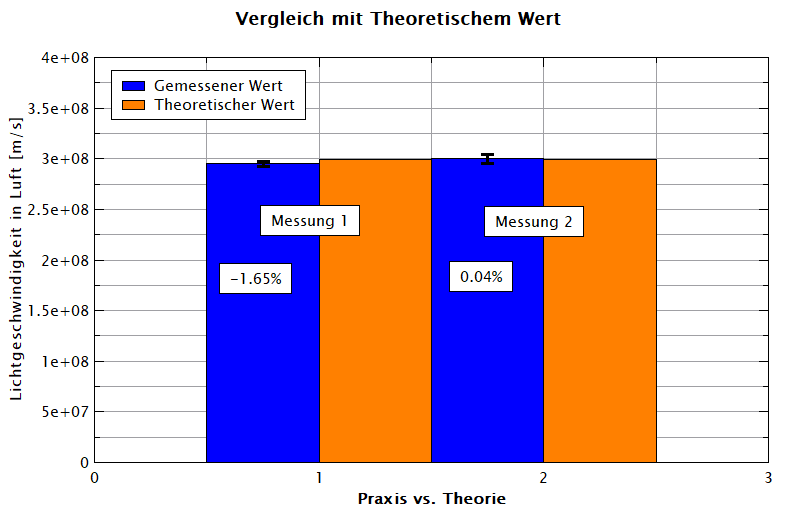
\includegraphics[width=\textwidth]{Vergleich_Messresultate.png}
\caption{Vergleich Messresultate}
\label{fig:Vergleich Messresultate}
\end{figure}
%%%%%%%%%%%%%%%%%%%%%%%%%%%%%%%%%%%%%%%%%%%%%%%%%%%%%%%%%%%%%%%%%%%%%%%%%%%%%

In Abbilung \ref{fig:Vergleich Messresultate} wird ersichtlich, dass sich unsere Messungen in der Nähe des gewünschten Wertes befinden. Die Messungen selbst zeigen eine sehr grosse Genauigkeit auf. Dies lässt darauf schliessen, dass sich ein systematischer Fehler eingeschlichen hat. Vermutlich waren unsere Distanzmessungen nicht ausreichend exakt. Der Messaufbau an sich konnte sehr einfach aufgebaut werden und hat uns in seiner Einfachheit überrascht. Mit ein paar Spiegeln und einem Drehspiegel ist es möglich die Lichtgeschwindigkeit zu bestimmen, dass war wirklich eine sehr interessante Erfahrung. Jedoch musste jede Distanz exakt eingestellt und ausgemessen werden. Die grösseren Distanzen haben wir mittels des Lasermessgerät eingestellt, evt. haben wir bei dessen Verwendung nicht präzise gearbeitet. Auch wäre es denkbar, dass wir bei der Verwendung der Mikrometerschraube fehlerhaft gearbeitet haben.\\
\\

Dieser Versuch war sehr interessant, da wir wirklich in der Lage waren die Lichtgeschwindigkeit zu bestimmen. Zuvor dachten wir, dass dazu ein komplexer Messaufbau nötig ist und waren erfreut, diese mittels so einfachen Mitteln durchführen zu können. Auch konnten wir bei diesem Versuch auf bereits angehäuftes Wissen, gewonnen aus vorhergegangenen Versuchen, wie z.B. über Optik zurückzugreifen.

